% !TEX root = ../main.tex

\chapter{Task Methodology}\label{ch:taskBackground}
This chapter will cover sections on how each part of the project will been carried out.
Useful notation is given in Section~\ref{sec:notation} which will allow us to describe a given sequence or set of sequences in a compact form.
We will also look at our specific instance of genetic algorithm that exists in the Axelrod Dojo~\cite{dojoV008} codebase.
Lastly Section~\ref{sec:solutionForm} looks at the what results we will expect from the analysis and the potential problems we want to mitigate.

\section{Notation}\label{sec:notation}
As described in Chapter 1 this work focuses on identifying best responses against the set of opponents in the Python Axelrod Library. The best responses are in a sequence format with a length of 200. In this Section we introduce a notation which will allow us to represent such sequences in a concise format.

Let \(S\in\{C, D\}^L\) where \(C\), \(D\) represents a cooperation, defection respectively.
\(L=200\) is used throughout this report.
Using the binary nature of the sequence we can split up sequences into blocks of consecutive move elements of the same type.
We will use \(B_i\) to denote the block after \(i\) changes of move type from the explicitly stated starting move type.
\begin{itemize}
    \item Every move in a block is of the same type, $C$ or $D$;
    the type is implicit based on whether \(i\) is even or not and what the starting move type was.
    \item We can use the notation \(|B_i|\) to denote the length of the \(i\)th block (number of moves within the block) in the sequence.\(|B_i| \in \mathbb{Z}\)
\end{itemize}

This means we can write a sequence as a series of blocks:
\[S= B_1 B_2,\ldots,B_n\]
A sequence can also be represented shorthand by specifying the starting move and the length of subsequent blocks:
\[S = C\ |B_1|,|B_2|,\ldots,|B_n|\ \quad \Rightarrow \quad S=\overbrace{C\ldots C}^{|B_1|}\overbrace{D\ldots D}^{|B_2|}\ldots\overbrace{(C|D)\ldots (C|D)}^{|B_n|} \]
We can also construct sequences from repetitions of a sequence of blocks when it makes sense:
\[C\ \big{(}|B_1|,|B_2|,\ \ldots,\ |B_m|\big{)}^{k}\ \quad \Rightarrow \quad \big{(}\small{\overbrace{C\ldots C}^{|B_1|}\overbrace{D\ldots D}^{|B_2|}\ldots\overbrace{D\ldots D}^{|B_m|}}\big{)}^{k-times}\]
The two notations can be combined to add starting and ending blocks to a repeating sequence (shown in the examples).

It is also possible to define sets of sequences by adding variables to parameters of the sequence.
Appropriate selection of parameters mean the length of sequences should not grow.
\[ \{Ci,l-i\} \quad i\in [a,b] \Rightarrow \{\underbrace{C\ldots C}_{a}\overbrace{D\ldots D}^{l-a},\ \underbrace{C\ldots C}_{a+1}\overbrace{D\ldots D}^{l-(a+1)},\ldots ,\ \underbrace{C\ldots C}_{b}\overbrace{D\ldots D}^{l-b}\} \]
For long sequences where there is no recognisable pattern it is typically easier to describe the solution.
Otherwise we use the notation to describe a sequence.
When we look at solutions there too long to write the sequence directly, in which case we may abbreviate in the following style: $C1,5,2,3,5,6,...=CDDDDDCCDDDCCCCCDDDDDD...$.

Examples:
\begin{align}
    C1,4,3,2 &= CDDDDCCCDD\\
    D(1,1)^{5} &= DCDCDCDCDC\\
    C1,(2,1)^{2},2,1 &= CDDCDDCDDC\\
    \{D[i,5-i]\} \quad i\in [2,4] &= \{DDCCC,\ DDDCC,\ DDDCC\}\\
\end{align}

To avoid confusion between a sequence for a given opponent, $S_{O_i}$, and the score for a given sequence we will define the score function $f(S_{O_i})$ as follows.
$$f(S_{O_i}):S_{O_i} \rightarrow [0,5]$$
This score function represents playing the sequence against the given opponent and calculating the score per turn over 200 turns.


\section{Customizing an Algorithm}\label{sec:buildingTheAlgorithm}
In order to generate a solution sequence we have to train against each Axelrod opponent.
Our implementation of a genetic algorithm has the following steps:
\begin{enumerate}
    \item Start with a predefined population, supplemented with randomly generated member until to size.
    \item Each member plays the given opponent with their sequence and returns with the average score per turn.
    \item Members of the population are ranked by this average score per turn and the highest scoring 25\% will be kept for the next round.
    The remaining 75\% are killed off.
    \item The remaining population will then be copied and these copies are mutated to create unique sequences before being merged back in to the main population.
    \item The remaining 50\% difference is then made up of mutated results of crossovers from members of the current population or random new members, depending on a random selection algorithm.\footnote{This algorithm had a bug which would change the size of the population in the first generation.
    This was fixed after Section~\ref{sec:conclusionOfApproach} was written.
    See: https://github.com/Axelrod-Python/axelrod-dojo/issues/43}
    \item A generation has now concluded.
    Repeat from step 2 until the desired number of generations are finished and a final best sequence is returned.
\end{enumerate}

\begin{figure}[ht]
    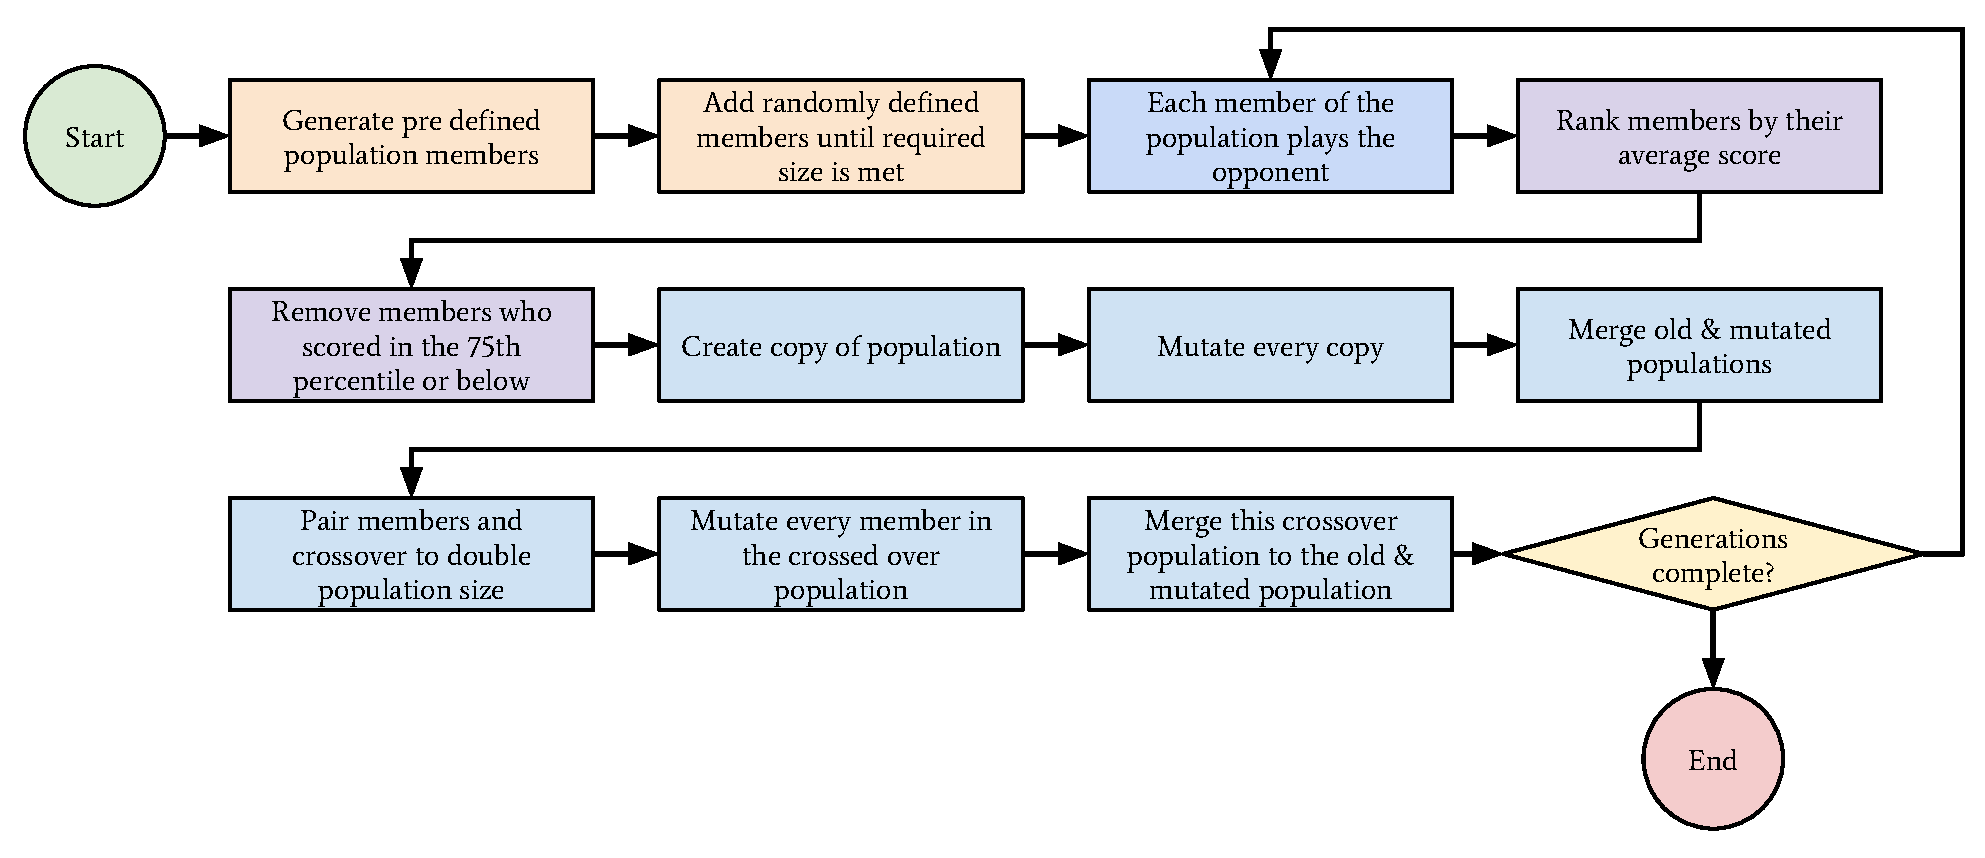
\includegraphics[width=1.0\textwidth, center]{./img/flows/custom_ga_cycle}
    \caption{High Level Genetic Algorithm Cycle. Extension of Figure~\ref{fig:genericGACycle}}\label{fig:customGAcycle}
\end{figure}

Figure~\ref{fig:customGAcycle} shows a flow diagram of our cycle.
This is the algorithm we will use in Chapter~\ref{ch:implementation} when analysing the algorithms parameters
The model means we can create a population of Cycler players, described in Section~\ref{sec:strategiesOfInterest}, and input a sequence of length 200 as a parameter to set off our genetic algorithm.
The subsequent inputs for the populations Cycler players will be created using the genetic mutation and crossover techniques, see Section~\ref{subsec:geneticAlgorithms} for details.

The looping will be the basis of creating the optimal strategy for each other opponent.
Each step is defined in the Axelrod Dojo \mintinline{python}{Population} and \mintinline{python}{CyclerParams} classes.
Rather than store all the functionality in one place we are able split up aspects of the flow to allow for flexibility in what type of population can be used.

\section{Solution Form}\label{sec:solutionForm}
In this research our goal will be to use the algorithm, described in Subsection~\ref{sec:buildingTheAlgorithm}, to produce an arbitrary sequence for an opponent, \(S_o\).
This sequence will represent the moves we should play against the opponent to get our largest potential score per turn for a single game of 200 turns.

This investigation focuses on sequences that will allow us to maximise our score overall, rather than just beating any given opponent.
An analogy of this concept is a team playing a football tournament, but instead of a knockout competition our team is placed in the standings based off the total goals they have scored across the tournament.
More real world applications of these results are discussed in Chapter~\ref{ch:conclusions}.

Each solution sequence is uniquely generated for each opponent.
If there are two similar opponents, say Grudger and Collective Strategy, these will be independently analysed and individual solutions will be generated.

If needed we may re-run analysis on some opponents if there are bugs that arise in the code.
In this case older results will be overwritten and previous analysis discarded.

When working with stochastic players, we will be seeding them in order to determine the best sequence.
Each stochastic player will be considered under a variety of seeds.
The motive to allow this to happen is explained described in Section~\ref{sec:stochasticOpponents}. Non-stochastic opponents will be seeded in the code, however there is no change in their behaviour because of this.

\section{Conclusion}
Here we have looked at the background required to answer a specific question, build a relevant model and understand what were looking for.
The concepts themselves are extensions to the basic models brought up in Chapter~\ref{ch:intro} and should allow us to provide relevant results in a uniform manner.

We have also looked at what problems may arise from certain areas of development, such as understanding what a best response for a stochastic opponents could be or how to represent a complex solution in a result.
Because of this premeditation of the problem and its components Chapters~\ref{ch:implementation} and~\ref{ch:results} will be more concise.

After we conclude the runtime of the GA and obtain a solution we will have an output sequence for each opponent.
These solution sequences can then be compared on how similar they are to each other;
what type of opponents and their corresponding `best scores' are and whether there are patterns to how to group strategies, Chapter~\ref{ch:results} contains further details.